\documentclass[journal]{IEEEtran}

\usepackage{blindtext}
\usepackage{amsmath}
\usepackage{amsfonts}
\usepackage{graphicx}
\usepackage{float}


\begin{document}
\title{Optimal Trajectory Exploration: Thrust Vectored Wing}
\author{Zachary Vogel, Ben Schroeder, Chris Gavin, Topher Pollard}
\markboth{December 2015}{Final Project: ECEN 5008}

\maketitle


\begin{IEEEkeywords}
    Thrust Vectored Wing, Optimization, Dynamics of Maneuvering Systems
\end{IEEEkeywords}

\section{Introduction}
In this project, we decided to explore the dynamics of a thrust vectored wing. Using these dynamics, we designed a trajectory for a Cuban Eight, and then simulated the dynamics attempting to follow said trajectory. Then, Professor Hauser's trajectory optimization code was used to optimize the system inputs to follow the trajectory, minimizing the mean squared error of the dynamic states. This gave us technical experience in working with dynamics and trajectories, which will be valuable in
our future controls engineering work.

\section{Background}
The model we built was largely based on two papers co-authored by Professor Hauser \cite{Jadbabaie}\cite{Franz}. Here, we define a point at which two input forces $f_x,\ f_z$ are applied. This point is defined as a distance, $l_\tau$ from the center of mass towards the tail of the airfoil moving along the vector in which the airfoil is pointed. Lift, drag, and velocity are defined in reference to the center of mass. Angle of attack, $\alpha$, is defined as the angle between the velocity vector,
$V$ and the direction the airfoil is pointed, aka the body frame. The flight path angle, $\gamma$ is defined as the angle between the x-axis of the inertial frame, and the velocity vector. The sum of these two angles defines $\theta$. An image describing this can be seen in figure 1.
\begin{figure}[h!]
    \centering
    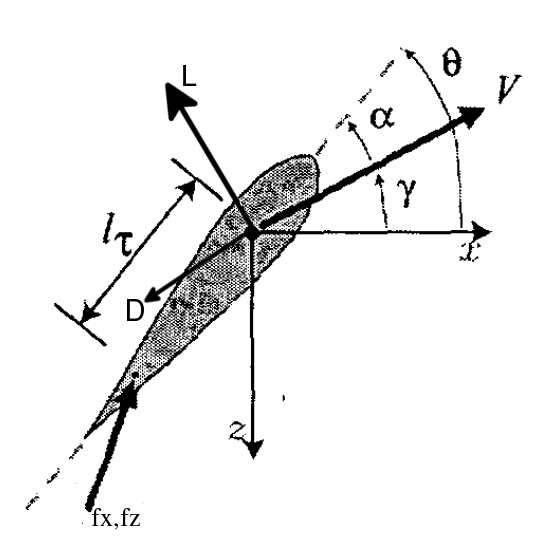
\includegraphics[width=0.45\textwidth]{wing_model.png}
    \caption{The thrust vectored wing we based our model on}
\end{figure}
\\
\indent The optimization that was performed with Professor Hauser's code was based on a Nonlinear Least Squares Trajectory\cite{Hauser}. The main idea being that we optimize a final trajectory based on a specified trajectory by minimizing a least squares functional. This was completely done for us, with our only task being to pass in dynamics, kinematics, and a desired trajectory. Our group also wrote code to build a trajectory. For this function, we define a velocity (V), $\gamma$, $\frac{dV}{dt}$
and $\frac{d\gamma}{dt}$. Then this function outputs a desired angle of attack, $\alpha$, and thrust vectors $f_x,f_z$. Note that $f_x$ can't be negative because it would be generating a thrust into the airfoil. Here, we write out the dynamics for the system:
\[\dot{V}=-\frac{D(V,\alpha)}{m}-g\sin(\gamma)+\frac{\cos(\alpha)}{m}f_x+\frac{\sin(\alpha)}{m}f_z\]
\[\dot{\alpha}=-\frac{L(V,\alpha)}{mV}+\frac{g}{V}\cos(\gamma)-\frac{\sin(\alpha)}{mV}f_x+\frac{\cos(\alpha)}{mV}f_z+\omega\]
\[\dot{\omega}=\frac{M(V,\alpha)}{J}+\frac{l_{\tau}}{J}f_z\]
\[\dot{\gamma}=\omega-\dot{\alpha}\]\\
\indent Where $\dot{\theta}=\omega$, $D(V,\alpha)$ is the drag force, $L(V,\alpha)$ is the lift force, $M(V,\alpha)$ is the moment due to aerodynamic forces, and $J$ is the moment of inertia. The drag, lift and moment equations are written:
\[L(V,\alpha)=\frac{1}{2}\rho V^2S3.256\alpha\]
\[D(V,\alpha)=\frac{1}{2}\rho V^2S(0.1716+2.395\alpha^2)\]
\[M(V,\alpha)=\frac{1}{2}\rho V^2S\bar{c}(-0.0999\alpha)\]
\\
\indent where, $\rho=1.2$kg/$m^3$, $\bar{c}=0.5$m, $m=12$kg, $g=0.6$m/$s^2$, $S=0.61$ $m^2$, $l_\tau=0.31$m and $J=0.24$ kg $m^2$. These values were experimentally determined in one of the papers by Professor Hauser\cite{Jadbabaie}. Here, $\rho$ is air density, $m$ is the mass of the airfoil, $g$ is the acceleration due to gravity, $S$ is the surface area of the airfoil, $l_\tau$ is the distance between the applied forces and the center of mass of the airfoil, J is the moment of inertia
about the center of mass, and $\bar{c}$ is the mean chord. Note that all of these dynamics are coupled, and that there is 4 states because of the acceleration due to gravity (otherwise 3 states would be sufficient). The last important thing is the kinematics which are defined below (our initial condition was $x=z=0$):
\[\dot{x}=v\cos(\gamma)\]
\[\dot{z}=-v\sin(\gamma)\]
\section{Simulation and Optimization}
\subsection{Constant Gain}
With all of our system defined, we needed to implement it into Professor Hauser's code for optimization. This involved finding the Jacobian of the dynamics equations and implementing them into dynamics.c. Once that was completed, we implemented the trim\_acc function which built the desired inputs ($f_x$ and $f_z$), and desired $\alpha$ from the desired $\gamma$ and velocity as well as their derivatives. This trim function also assumed that $\dot{\omega}=0$ and that $\dot{\alpha}=0$. This was
accomplished using the fsolve function in Matlab. This made it relatively easy to implement a Cuban Eight in sections and attach them together. We defined a constant velocity and then adjusted $\gamma$ to implement a Cuban eight. Starting at the bottom of the curved section at $\gamma=0$, we change $\gamma$ linearly to $\gamma=\pi$. Then, for the next section we transition linearly from $\gamma=\pi$ to $\gamma=\frac{5\pi}{4}$ back to $\gamma=\pi$. By varying $\gamma$ from $\pi$ to $0$ then
from $0$ to $-\frac{\pi}{4}$ back to $0$ and you should end close to the starting point.\\
\indent Having found the variables to determine our trim trajectory, we ran drive\_sys.m which generated the desired trajectory and simulated the dynamics on that trajectory with a constant gain. The linear quadratic regulator gains that were used in this system were defined in QR\_params.h. For one trial, these were set to $Qr[]=\{10.0,50.0,20.0,40.0\}$, and $Rr[]=\{0.1,0.1\}$. The output of the drive\_sys.m can be seen below, note the inputs that resulted in the actual graphs were
the trim calculated $f_x$ and $f_z$.
\begin{figure}[h!]
    \centering
    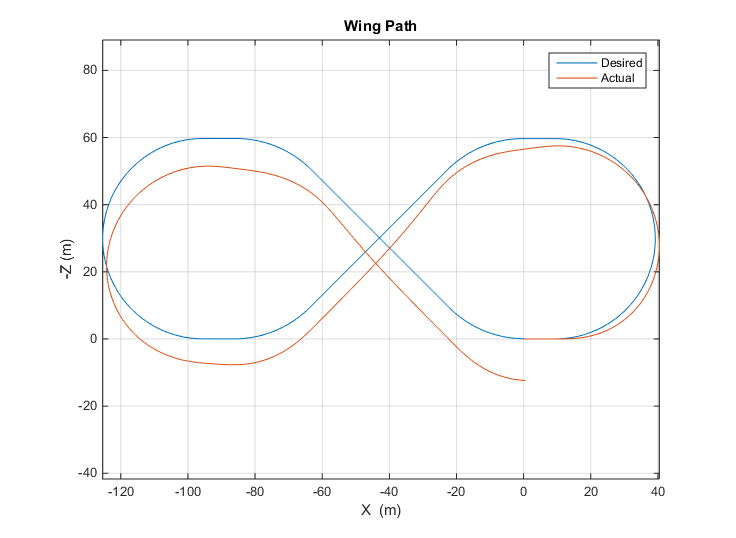
\includegraphics[width=0.5\textwidth]{Flight_Path_Constant_Gain.png}
    \caption{The flight path using a constant gain}
\end{figure}\\
\indent As is evident, the dynamics tried to follow the desired trajectory, but failed. At this point we decided to look at several of the states to see if we could figure out why. First, we looked at the velocity graph in figure 3. This illustrates why the error in flight path happened. The velocity was almost always above what the desired value was because of this, flight path error accumulated in the descent section. This means our simulation showed the airfoil flying farther downwards
in the z direction than it should have, which resulted in an end position further down than desired.
\begin{figure}[h!]
    \centering
    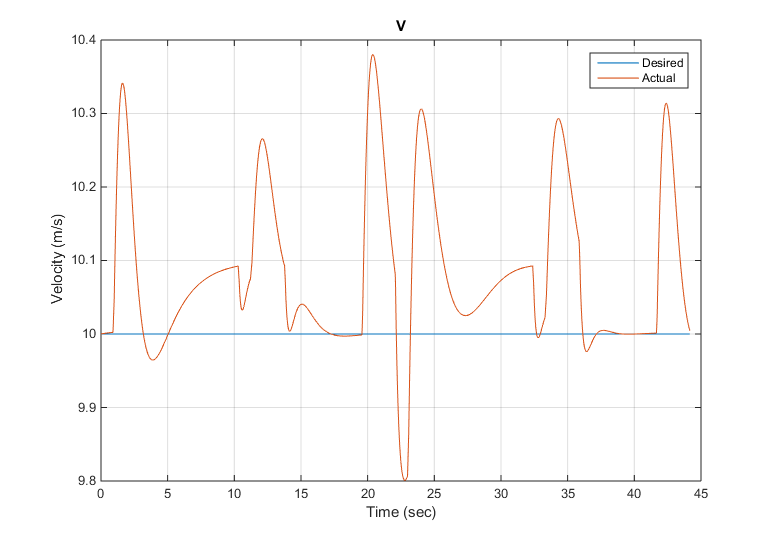
\includegraphics[width=0.5\textwidth]{V_Constant_Gain_LQR.png}
    \caption{The non-optimized velocity during a Cuban Eight, note that the total error is positive}
\end{figure}
\indent We also examined a few other things to see if we could account for the error in flight path. In figure 4, we see $\gamma$ desired and actual. This seemed to follow pretty well, but there are some overshoots that result in some of the discrepencies that we see. The slight overshoots cause the system to angle downwards a few degrees more than it should which results in our final position being significantly below the starting position. For figure 5, we see the $\omega$ as a function of time.The important thing to notice for that is the overshoot on every instantaneous change happening in the system. This was too hard to interpret, but shows that there was a large error between the desired and actual state.
\begin{figure}[H]
    \centering
    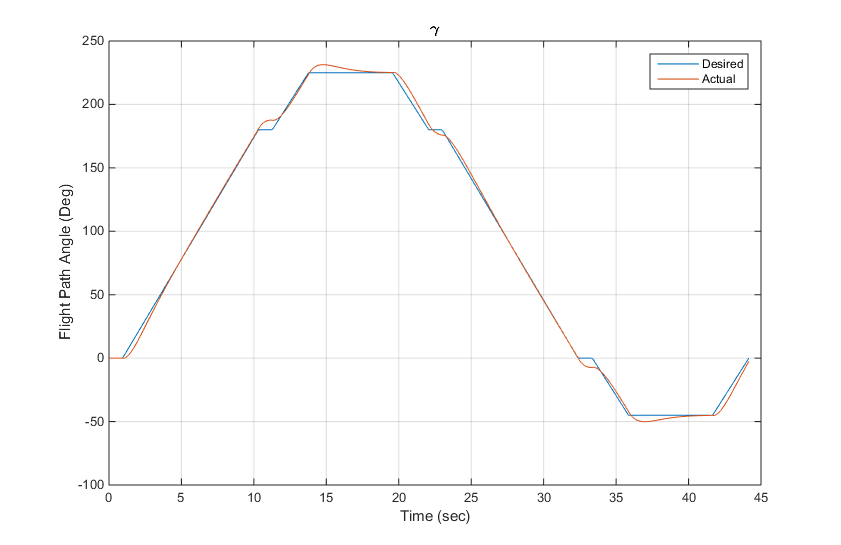
\includegraphics[width=0.5\textwidth]{Gamma_Constant_Gain_LQR.png}
    \caption{The actual $\gamma$ vs desired $\gamma$. The errors here are not huge, but do make a significant difference in the final position.}
\end{figure}
\begin{figure}[H]
    \centering
    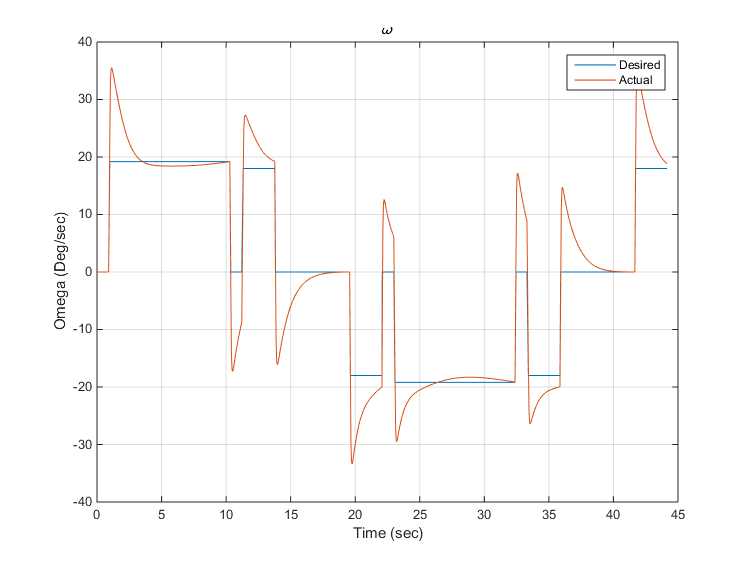
\includegraphics[width=0.5\textwidth]{Omega_Constant_Gain_LQR.png}
    \caption{$\omega=\dot{\theta}$ The derivative of the angle of the plane relative to the Inertial plane}
\end{figure}
\indent The final state we examined was the angle of attack, which is directly related to the lateral acceleration. The actual output looks like it was put through a low pass filter. The angle of attack peaks at about 20, which is at least reasonable. Also, note that this is largely responsible for the lift of our model, which is why its peak deviation from zero is when we are changing in the z coordinate the most.
\begin{figure}[H]
    \centering
    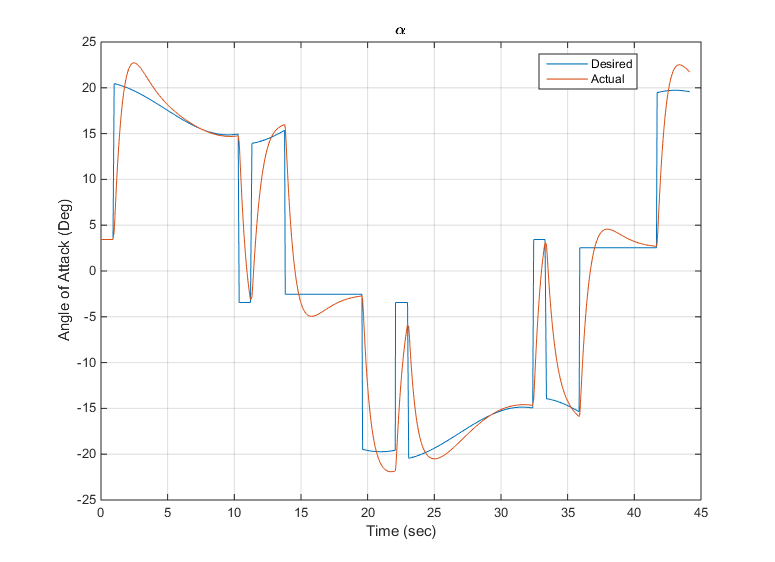
\includegraphics[width=0.5\textwidth]{Alpha_Constant_Gain_LQR.png}
    \caption{Angle of attack, $\alpha$, looks as if a low pass filter was applied.}
\end{figure}
\indent The last things we looked at to examine the discrepancy in our actual flight path were the inputs $f_x$ and $f_z$ seen in figures 6 and 7. Starting with $u_1=f_x$, note that it does in fact go negative at one point in the graph, which is impossible. Also, notice the spikes followed by negative error when every there was a rapid change in the desired trajectory. These probably resulted in some error, but are somewhat unavoidable, as we will see in the optimized system. Finally,
observe the $u_2=f_z$ input. Any time there is a pseudo-instantaneous change, the input overshoots by a ton and then tries to correct itself. This would cause issues in a real system were you would need some kind of saturation to prevent your desired inputs from breaking the system's thrust generator.
\begin{figure}[h!]
    \centering
    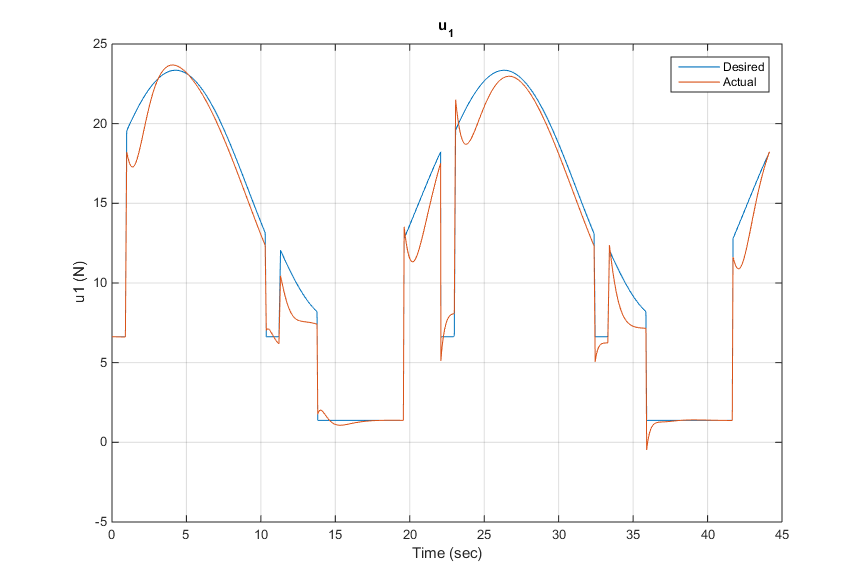
\includegraphics[width=0.5\textwidth]{U1_Constant_Gain_LQR.png}
    \caption{The U1 input, $f_x$. Note that it goes negative at one point in the graph which isn't allowed.}
\end{figure}
\begin{figure}[h!]
    \centering
    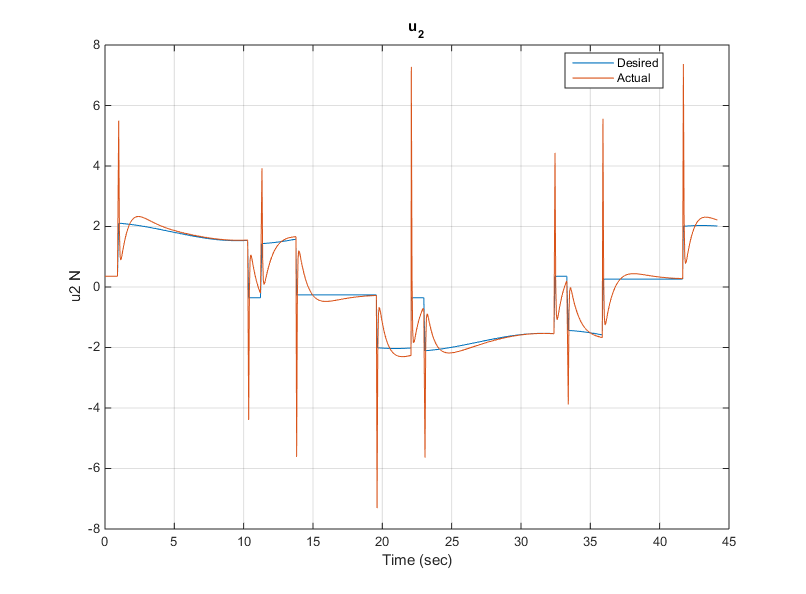
\includegraphics[width=0.5\textwidth]{U2_Constant_Gain_LQR.png}
    \caption{The U2 input, $f_z$. This input is allowed to be negative so that we have a $\pi$ range of vectored thrust}
\end{figure}\\
\indent The final thing to note about the constant feedback system is that the LQR was based on a linearization about the starting point, $(x,y)=(0,0)$. This is the main reason states don't follow their desired paths, and will largely be fixed by the optimization algorithm.
\subsection{Optimized Gain}
Now that we had a nice desired trajectory, we were able to run the optimization algorithm to give us a nice output. As can be seen in figure 9, the optimally calculated flight path is very close to the desired. It differs by around $0.1$m at most over the whole Cuban Eight. This is exactly what we were looking for, but we still wanted to examine the inputs and states to get an idea of what the optimization algorithm did.
\begin{figure}[H]
    \centering
    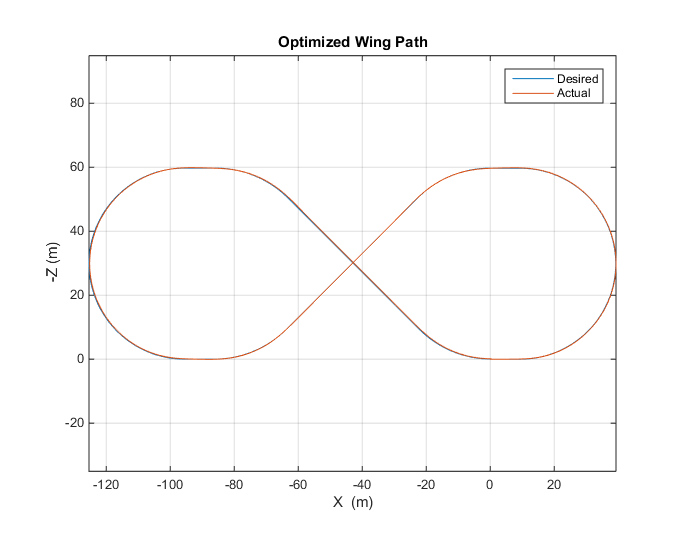
\includegraphics[width=0.5\textwidth]{Flight_Path_Optimized.png}
    \caption{The optimized gain flight path. As you can see it follows the desired trajectory extremely well.}
\end{figure}
\indent Looking at the inputs in figure 10, there are several important things to note. First, the $f_x$ input, $u_1$, no longer goes negative. This meant we didn't have to include a saturation or event effect on the optimization code. Second, the $f_z$ input, $u_2$ still has trouble responding to instantaneous changes in the desired trajectory, but overshoots less than in the unoptimized version. In fact, the overshoot is now only about $2$ times the instantaneous change as opposed to $2.5-4$ times the instantaneous change in the unoptimized version. The other problem with the $f_z$ input is that it still exhibits weird behavior just outside of these jumps. I think a minor low-pass filter could be applied to the desired $f_z$ to get a more realistic change in the variable.
\begin{figure}[H]
    \centering
    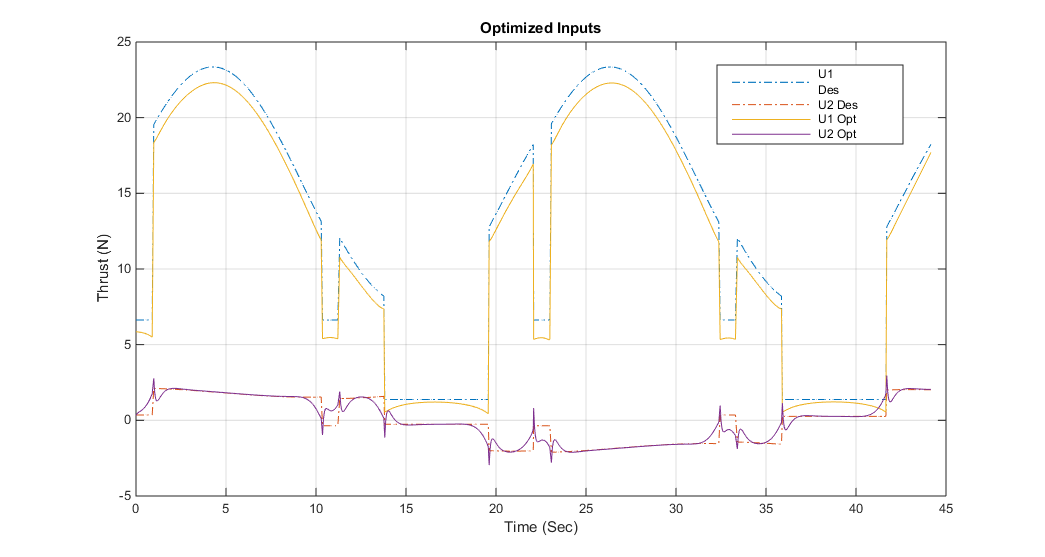
\includegraphics[width=0.5\textwidth]{Inputs_Optimized.png}
    \caption{The two optimized inputs relative to the desired. Note that $f_x$ no longer goes negative at around 36 seconds.}
\end{figure}
Finally, we examined the states of the system under the optimized inputs. First, we noticed that the actual velocity was extremely close to the desired constant velocity. It only really differed by around $0.1$ m/s which we think is quite good. The optimized inputs also followed the $\gamma$ near flawlessly, showing very little error between the actual and desired states. Despite this, the angle of attack and $\omega$ struggled to follow the desired states. Both state differences had minimal
error in the constant regions, but couldn't handle the rapid desired change at various points. This resulted in different kinds of compensation. The angle of attack fixed this by beginning to change slowly before and after the large jumps. This meant the $\alpha$ error was positive before positive jumps and negative just after the jump. That is not how the $\omega$ state handled the error. The $\omega$ state accumulated a ton of positive error on positive instantaneous jumps, but corrected for this by getting a ton of negative error on the negative jumps. Both of these effects were non-causal and due to the optimization algorithm.
\begin{figure}[H]
    \centering
    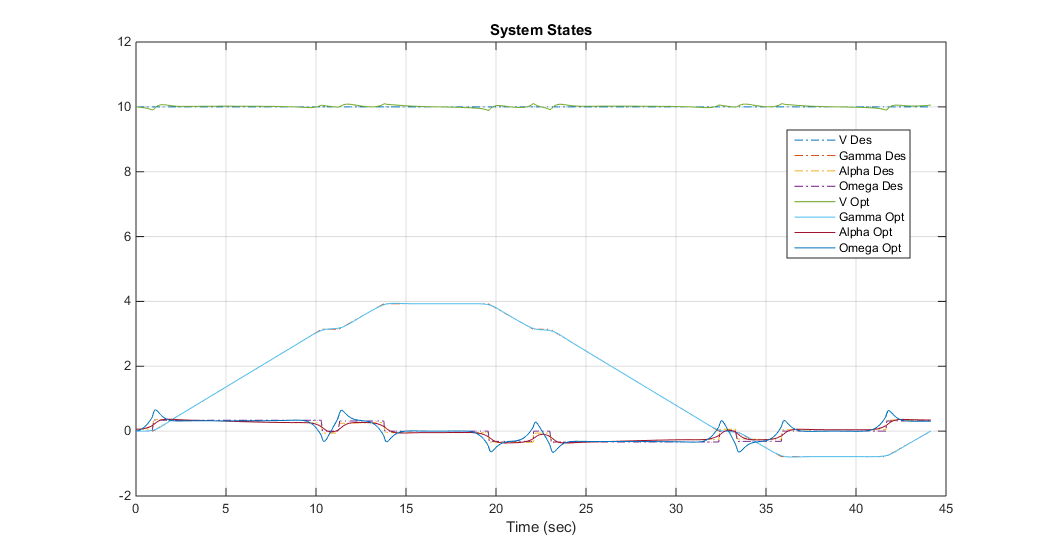
\includegraphics[width=0.5\textwidth]{Optimized_States.png}
    \caption{The states after optimization. Note that the velocity and $\gamma$ are almost perfectly following their desired states. The $\omega$ and $\alpha$ do not do this, still not being able to handle the fast changes in the desired values. The $\omega$ state compensates for this by overshooting on both sides of the fast changes, while the angle of attack compensates by basically applying a low pass filter to the desired change, and being non-causal.}
\end{figure}

\section{Conclusion}
Through this project, we have explored the dynamics of a 2 dimensional airfoil by exploring how it follows a given trajectory under constant gain and optimized feedback. This taught us a lot about the dynamics of this relatively simple system and how to explore properties of systems such as this. A continuation of this project could explore the second order derivatives of this system, adding another axis of motion, and/or an analysis on how realistic the optimized states are in a real system.
Overall, we feel this was an interesting project that furthered our understanding of dynamics and trajectory tracking.
\begin{thebibliography}{9}
    \bibitem{Jadbabaie}
        Jadbabaie, A., \& Hauser, J. (n.d.). Control of a thrust-vectored flying wing: A receding horizon? LPV approach. International Journal of Robust and Nonlinear Control Int. J. Robust Nonlinear Control, 869-896.
    \bibitem{Franz}
        Franz, R., \& Hauser, J. (n.d.). Optimization based paramter indentification of the Caltech ducted fan. Proceedings of the 2003 American Control Conference, 2003.
    \bibitem{Hauser}
        Hauser, J. (2012, December 1). \emph{Nonlinear Least Squares Trajectory Exploration}. Lecture presented in CU Boulder, Boulder.
\end{thebibliography}



\end{document}
